\begin{answer}
\begin{figure}[htb]
    \begin{subfigure}{0.5\linewidth}
        \centering
        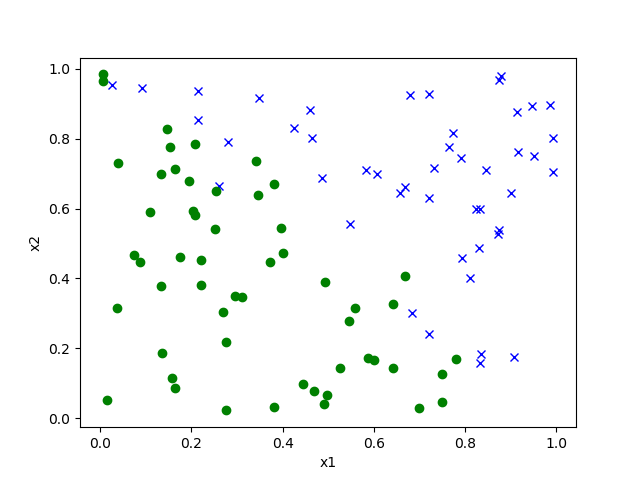
\includegraphics[width=\linewidth]{tex/a.png}
        \subcaption*{Dataset A}
    \end{subfigure}
    \begin{subfigure}{0.5\linewidth}
        \centering
        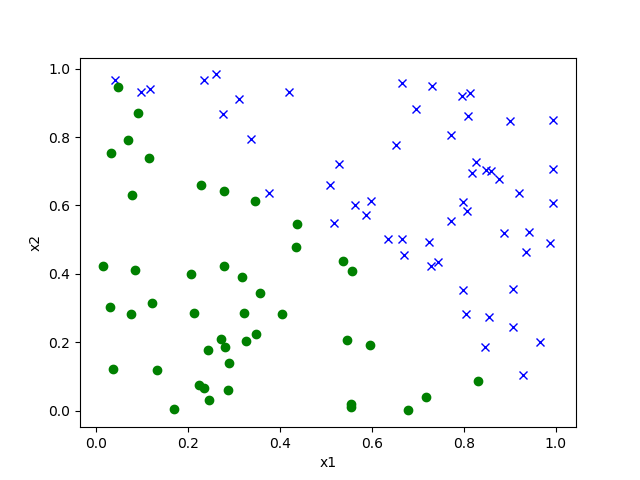
\includegraphics[width=\linewidth]{tex/b.png}
        \subcaption*{Dataset B}
    \end{subfigure}
    
\end{figure}
The dataset B is perfectly linear separable. In this case, when the logistic regression finds a decision boundary that can separate the dataset perfectly, the algorithm can decrease the negative log-likelihood function by multiplying the $\theta$ by a arbitrary number. However, multiplying the $\theta$ by a number doesn't change the decision boundary. Like the functional margin of SVM, we can make the $\theta$ arbitrarily large without really changing anything meaningful. 
Logistic regression can converge on the dataset A, because that dataset is not linearly separable.
\end{answer}
